\documentclass{stex}
\libinput[smglom/meta-inf]{preamble}
\libinput[COPE]{cope-preamble}
\begin{document}
\begin{smodule}[title={Redundant Visited Node}]{redundant-visited-node}
  \usemodule[smglom/search]{mod?search-algorithm}
  \usemodule[smglom/didactics]{mod?common-error-pattern}
  \usemodule[smglom/didactics]{mod?task-constraint}
  \usemodule[smglom/didactics]{mod?learning-task}

  \symdecl*{redundant-visited-node}


\begin{sdefinition}
  \Definame{redundant-visited-node} is a \sr{CEP}{common error pattern} in \sn{graph} \sr{search algorithm}{search} \sr{learning task}{tasks} where a previously visited \sn{node} is revisited and explicitly mentioned again, despite the \sns{task constraint} stating that visited nodes should not be repeated. 
\end{sdefinition}

\begin{sparagraph}
  This often occurs when a search algorithm fails to properly track visited nodes or when the implementation does not enforce the requirement to avoid re-exploration. As a result, the search may produce incorrect paths, redundant computations, or inefficient traversal of the graph.
\end{sparagraph}



%%%%%%%%%%%%%%%%%%%%%%%%%%%%%%%%%%%%%%%%%%%%%%%%%%%%%%%%%%%%
%%%%% DIAGNOSIS %%%%%%%%%%%%%%%%%%%%%%%%%%%%%%%%%%%%%%%%%%%%
%%%%%%%%%%%%%%%%%%%%%%%%%%%%%%%%%%%%%%%%%%%%%%%%%%%%%%%%%%%% 
%% For Human Diagnosis:
%%%% How to detect the pattern
%%%% What are the indicators of the pattern
%%%% What are the symptoms of the pattern
%%%% What are (possible) causes of the pattern
%% Automated Diagnosis: 
%%%% References to resulting tests (Unit-Test-Suites etc.)

\begin{sparagraph}[title=Diagnosis]
  \begin{itemize}
  \item \textbf{Repeated Node Labels:} Nodes are explicitly mentioned multiple times in the search path.
  \item \textbf{Inconsistent Path Length:} The path length is longer than expected due to revisiting nodes.
  \item \textbf{Redundant Computations:} Nodes are processed multiple times, leading to inefficiencies.
  \end{itemize}
\end{sparagraph}

%%%%%%%%%%%%%%%%%%%%%%%%%%%%%%%%%%%%%%%%%%%%%%%%%%%%%%%%%%%%
%%%%% EXAMPLE %%%%%%%%%%%%%%%%%%%%%%%%%%%%%%%%%%%%%%%%%%%%%%
%%%%%%%%%%%%%%%%%%%%%%%%%%%%%%%%%%%%%%%%%%%%%%%%%%%%%%%%%%%%
%% 1) Helps educators to understand/detect the error pattern
%% 2) Serves as KC-EXA feedback (Knowledge about Concept - Examples illustrating concepts)

\begin{sexample}[title="Redundant Visited Node Error"]

  The following graph shows a directed graph with nodes $A$ to $F$ and edges with weights 1. The task is to find a path from $A$ to $F$ using a breath-first search algorithm. The algorithm should avoid revisiting nodes that have already been visited.
  \begin{center}
    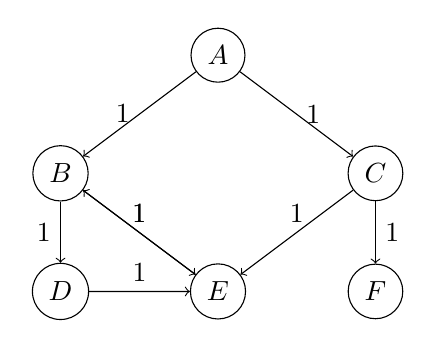
\begin{tikzpicture}[yscale=1.5]
    \node[circle,draw] (A) at (0,0) {$A$};
    \node[circle,draw] (B) at (-2,-1) {$B$};
    \node[circle,draw] (C) at (2,-1) {$C$};
    \node[circle,draw] (D) at (-2,-2) {$D$};
    \node[circle,draw] (E) at (0,-2) {$E$};
    \node[circle,draw] (F) at (2,-2) {$F$};
    \draw[->] (A) --node[left] {1} (B);
    \draw[->] (A) --node[right] {1} (C);
    \draw[->] (B) --node[left] {1} (D);
    \draw[->] (B) --node[above] {1} (E);
    \draw[->] (C) --node[above] {1} (E);
    \draw[->] (C) --node[right] {1} (F);
    \draw[->] (E) --node[above] {1} (B); % Redundant visit error
    \draw[->] (D) --node[above] {1} (E);
    \end{tikzpicture}
\end{center}


\begin{align*}
  \text{Correct:} \quad & A B C D E F \\
  \text{With (one) redundant visit error:} \quad & A B C D E \textcolor{red}{E} F \\
  \text{Complete redundant visit error:} \quad & A B \textcolor{red}{A} C \textcolor{red}{A} \textcolor{red}{B} D \textcolor{red}{B} E \textcolor{red}{B} \textcolor{red}{A} \textcolor{red}{C} \textcolor{red}{E} \textcolor{red}{C} F \textcolor{red}{C}
  \end{align*}

\end{sexample}



%%%%%%%%%%%%%%%%%%%%%%%%%%%%%%%%%%%%%%%%%%%%%%%%%%%%%%%%%%%%
%%%%% FEEDBACK %%%%%%%%%%%%%%%%%%%%%%%%%%%%%%%%%%%%%%%%%%%%%
%%%%%%%%%%%%%%%%%%%%%%%%%%%%%%%%%%%%%%%%%%%%%%%%%%%%%%%%%%%%
%% Default Feedback Messages for different feedback types

\begin{sfeedback}

  % Knowledge of Result
  \feedback[type=KR, form=T]{Your answer is correct.}
  \feedback[type=KR, form=F]{Your answer is incorrect.}

  % Knowledge about task constraints (KTC)
  \feedback[type=KTC, form=i]{The task constraints require that each node is visited only once during the search. Adhering to this limitation is essential to maintain algorithm efficiency and prevent infinite loops.}
  \feedback[type=KTC, form=r]{Reflect on how your implementation enforces the rule that each node is visited only once. How have you ensured that this constraint is strictly followed to maintain efficiency and avoid infinite loops?}
  
  
  % Knowledge about concepts - Explanation on subject matter (KC-EXP)
  \feedback[type=KC, form=i]{Graph search algorithms depend on the principle of tracking visited nodes. This concept ensures that each node is processed only once, thereby preserving the integrity and systematic nature of the search.}
  \feedback[type=KC, form=r]{Consider the role of tracking visited nodes in graph search algorithms. In what ways does your solution embody this principle, and how does it support a systematic and efficient search?}
  
  % Knowledge about mistakes (KM)
  \feedback[type=KM, form=i]{The error occurs when a node that has already been visited is processed again. This mistake leads to redundant computations and may result in incorrect paths being identified in the search algorithm.}
  \feedback[type=KM, form=r]{Examine your algorithm for signs of processing a node more than once. What indicators in your code or output suggest that redundant computations might be occurring?}
  
  
  % Knowledge about how to proceed (KH)
  \feedback[type=KH, form=i]{To correct this error, verify that your implementation marks each node as visited immediately upon processing. Adjust your tracking mechanism to ensure that no node is revisited once it has been accounted for.}
  \feedback[type=KH, form=r]{What modifications can you explore to ensure that nodes are marked as visited immediately upon processing? How would these changes help you avoid revisiting nodes in your algorithm?}

  % Knowledge about meta-cognition (KMC)
  \feedback[type=KMC, form=i]{After implementing your solution, review the task description to confirm that all constraints are properly met. Systematically trace your code and the calculated results to verify that every step aligns with the specified requirements. This careful review is essential for identifying and correcting subtle mistakes in your implementation.}
  \feedback[type=KMC, form=r]{After completing your implementation, what systematic approach will you use to review your code and verify that every step aligns with the task constraints? How will you ensure that subtle errors are not overlooked?}
\end{sfeedback}


%%%%%%%%%%%%%%%%%%%%%%%%%%%%%%%%%%%%%%%%%%%%%%%%%%%%%%%%%%%%
%%%%% LEARNER MODEL %%%%%%%%%%%%%%%%%%%%%%%%%%%%%%%%%%%%%%%%
%%%%%%%%%%%%%%%%%%%%%%%%%%%%%%%%%%%%%%%%%%%%%%%%%%%%%%%%%%%%
% How to trigger the LM if the error pattern is detected





\end{smodule}
\end{document}

%%% Local Variables:
%%% mode: latex
%%% TeX-master: t
%%% End:
